\documentclass[11pt, oneside]{article} 
\usepackage{geometry}
\geometry{letterpaper} 
\usepackage{graphicx}
	
\usepackage{amssymb}
\usepackage{amsmath}
\usepackage{parskip}
\usepackage{color}
\usepackage{hyperref}

\graphicspath{{/Users/telliott_admin/Tex/png/}}
% \begin{center} 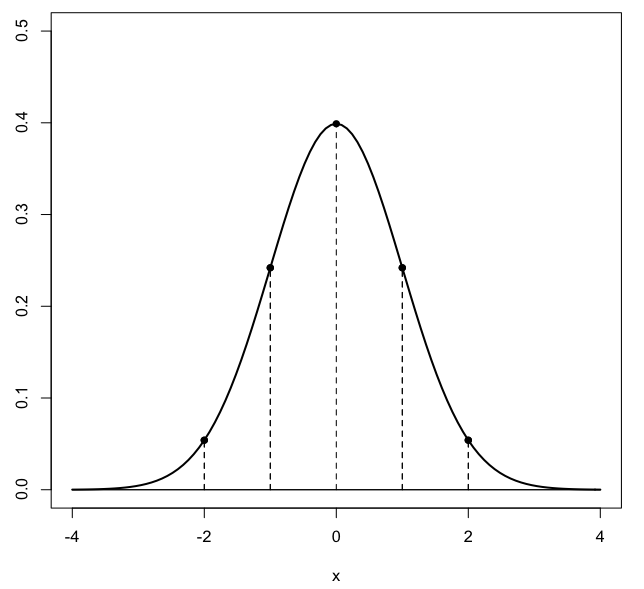
\includegraphics [scale=0.4] {gauss3.png} \end{center}

\title{Convergence}
\date{}

\begin{document}
\maketitle
\Large

\subsection*{bounded, monotone sequences}

We combine the previous concepts of a bounded monotone sequence and convergence:

\textbf{Axiom}  (Monotone Sequence Property). \emph{Any bounded monotone sequence converges.}

Beck:
\begin{quote}This axiom (or one of its many equivalent statements) gives arguably the most important property of the real number system; namely, that we can, in many cases, determine that a given sequence converges without knowing the value of the limit. In this sense we can use the sequence to define a real number.\end{quote}


\subsection*{theorem}

$\bullet$  A bounded monotonic increasing sequence converges, and it converges to its least upper bound.

\subsection*{proof}

Let $\alpha$ be the least upper bound of the sequence.

Given $\epsilon > 0$, we will show that all the terms of the sequence after some finite number of initial terms are in the interval $(\alpha - \epsilon, \alpha + \epsilon)$.

$\circ$  Since $\alpha + \epsilon$ is an upper bound of the sequence, all the terms certainly satisfy $a_n < \alpha + \epsilon$.

$\circ$  And since $\alpha - \epsilon$ is \emph{not} an upper bound of the sequence, we must have $a_N > \alpha - \epsilon$ for some $N$.

$\circ$  But then all the later terms $a_n$ (for $n > N$)  will satisfy $a_n > \alpha - \epsilon$ (by the monotonic property), and so we have our condition for convergence.

\subsection*{restated theorem}

If $(a_n)$ is a monotone sequence of real numbers, then $(a_n)$ is convergent if and only if it is bounded.

\subsection*{expanded proof}

Let $(a_n)$ be a monotone sequence.

$\Rightarrow$

Suppose that $(a_n)$ is convergent.  We showed previously that any convergent sequence is bounded.

$\Leftarrow$

There are two symmetric cases, increasing and decreasing.  We consider only the first.

Suppose that $(a_n)$ is an increasing sequence that is bounded.  We look at the set $\mathbf{a} = \{ a_n: n \in \mathbb{N} \}$.  The set $\mathbf{a}$ is also bounded.  By the completeness property, it has a least upper bound or supremum $L \in \mathbb{R}$.

Let $\epsilon > 0$ be given.  Since $L$ is the supremum of $\mathbf{a}$, $L - \epsilon$ cannot be an upper bound for the set so $\exists \ a_N$ such that $L - \epsilon < a_N$.

Since $a_n$ is increasing, we have that for all $n \ge N$, $a_N \le a_n$ so:
\[ L - \epsilon < a_N \le a_n \le L < L + \epsilon \]
\[ L - \epsilon < a_n < L + \epsilon \]
\[ |a_n - L| < \epsilon \]

This proves that $(a_n)$ converges to $L$.

$\square$

\end{document}